% \section{Multi-Agent Chatbot and Recommendation System}
\section{Multi-Agent Chatbot System with Goal-Oriented Question Suggestion}
\label{sec:multi_agent_architecture}

% The entire system is organized under a multi-agent architecture, where each agent is a specialized software module powered by a large language model (LLM) and responsible for a distinct subtask. This design enables the system to handle complex workflows in a flexible and modular manner. The overall architecture is illustrated in Figure~\ref{fig:architecture}. In addition to the product knowledge graph, the system comprises two main components: the \textit{Recommendation Component} and the \textit{Chatbot Response Generation Component}.

% The integration of the Question Suggestion Component and the Response Generation Component enables a seamless conversational flow. Each response not only addresses the user's query but also introduces follow-up suggestions aligned with business goals, forming an intelligent and proactive interaction loop.


The system is built upon a multi-agent architecture, in which each agent is a specialized software module powered by a large language model (LLM) and dedicated to a specific subtask. This modular design allows the system to handle complex conversational workflows in a flexible and coordinated manner. The overall architecture is depicted in Figure~\ref{fig:architecture}. All LLM-based agents are implemented with the Gemini 2.5 Flash model, selected for its efficiency and strong reasoning capabilities in multi-turn dialogue. For embedding generation, we use Google’s \texttt{text-embedding-004} model, as described in Section~\ref{sec:chatbot_response}.

In addition to the product knowledge graph, the system consists of two primary components: the \textit{Question Guidance Component} and the \textit{Chatbot Response Generation Component}. Their integration enables a seamless conversational flow, where each response not only answers the user's question but also introduces follow-up suggestions aligned with business objectives, establishing an intelligent and proactive interaction loop.

% Toàn bộ hệ thống được thiết kế theo kiến trúc đa tác tử (multi-agent), nơi mỗi tác tử là một thực thể phần mềm chuyên biệt, được hỗ trợ bởi LLM, đảm nhiệm một nhiệm vụ cụ thể. Kiến trúc này cho phép hệ thống xử lý các luồng công việc phức tạp một cách linh hoạt và có tổ chức. Hình \ref{fig:architecture} mô tả luồng hoạt động tổng thể của hệ thống. Ngoài thành phần đồ thị tri thức, hai thành phần chính khác trong hệ thống là: Thành phần Gợi ý (Recommender Component) và Thành phần Chatbot (Chatbot Component).


\begin{figure}[!t]
    \centerline{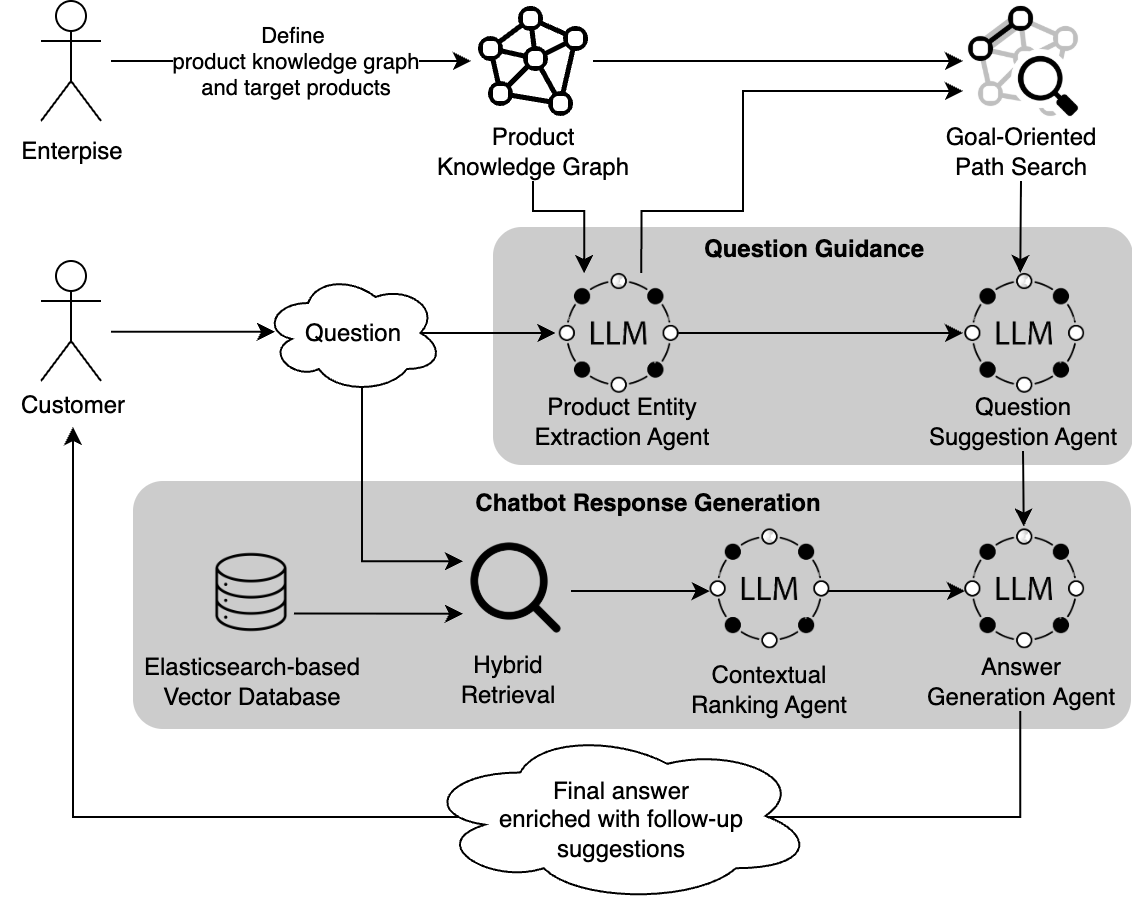
\includegraphics[width=0.5\textwidth]{Figure/overall_flow.png}}
    \caption{The overall architecture of the multi-agent chatbot with goal-oriented question suggestion.}
    \label{fig:architecture}
\end{figure}


\subsection{Question Guidance Component}

This component is responsible for generating suggestion questions to guide the conversation toward business-defined goals. It consists of two LLM-based agents: the \textit{Product Entity Extraction Agent} and the \textit{Question Suggestion Agent}.


% \subsection{Thành phần Gợi ý}
% Thành phần này chịu trách nhiệm tạo ra các câu hỏi gợi ý để dẫn dắt cuộc hội thoại. Nó bao gồm Tác tử Nhận dạng Thực thể và Tác tử Gợi ý Tự nhiên.

\textbf{Product Entity Extraction Agent:} When the user poses a query, this agent identifies the names of smartphone products mentioned in the utterance. It uses a large language model prompted for the Named Entity Recognition (NER) task. The extracted product names are then matched against the product knowledge graph using fuzzy search techniques to locate the corresponding source nodes.

% \textbf{Tác tử Nhận dạng Thực thể (NER Agent):} Khi người dùng đặt câu hỏi, tác tử này có nhiệm vụ trích xuất tên của các sản phẩm smartphone được đề cập. Agent là một LLM với prompt được thiết kế cho tác vụ Named Entity Recognition (NER). Tên sản phẩm được trích xuất sau đó được đối chiếu với cơ sở dữ liệu bằng kỹ thuật tìm kiếm mờ (fuzzy search) để xác định chính xác nút thực thể nguồn trong đồ thị tri thức.

\textbf{Question Suggestion Agent:} This agent receives as input a set of high-scoring paths from the knowledge graph traversal algorithm. For each path, it extracts a triplet consisting of the source product, the next product along the path, and the semantic relationship connecting them. Based on this triplet, the agent generates two outputs: a \textit{rationale sentence} and a \textit{follow-up question}. 

The \textit{rationale sentence} provides a natural-language explanation of why the next product is relevant. For example: \textit{“Alongside the Samsung Galaxy S25, another phone in the same price range of 20–25 million VND that you might find interesting is the iPhone 15.”}

The \textit{follow-up question} is a targeted inquiry about the suggested product, designed to encourage further user engagement. For instance: \textit{“Would you like to explore how the iPhone 15’s performance compares to the previous model?”}

% \textbf{Tác tử Gợi ý Tự nhiên (Natural Recommendation Agent):} Tác tử này nhận đầu vào là các đường đi tối ưu từ thuật toán tìm kiếm trên đồ thị tri thức. Với mỗi đường đi, nó lấy ra bộ ba dữ liệu bao gồm: sản phẩm nguồn, sản phẩm ngay sau sản phẩm nguồn trên đường đi, và quan hệ giữa hai sản phẩm này. Dựa trên thông tin này, nó tạo ra một lời giải thích gợi ý và một câu hỏi gợi ý. \textbf{Lời giải thích} là một câu văn tự nhiên giải thích lý do tại sao sản phẩm tiếp theo lại liên quan. Ví dụ: \textit{"Bên cạnh chiếc Samsung Galaxy S25, một chiếc điện thoại khác trong cùng tầm giá 10-11 triệu mà bạn có thể quan tâm là iPhone 15."}
% \textbf{Câu hỏi gợi ý} là một câu hỏi cụ thể về sản phẩm được gợi ý, khuyến khích người dùng khám phá thêm. Ví dụ: \textit{"Bạn có muốn tìm hiểu về cấu hình của iPhone 15 có cải tiến gì so với phiên bản trước không?"}

On the chatbot interface, the \textit{rationale sentence} is appended directly to the previous system response, while the \textit{follow-up questions} are displayed below as clickable options for the user. This design enables a seamless connection between the suggested product (e.g., iPhone 15) and the user's current interest (e.g., Samsung Galaxy S25) as they share the same attribute value, such as price range. The follow-up questions, however, are not constrained to this specific attribute; they are designed to encourage broader exploration of the suggested product across multiple dimensions.

% Trên giao diện chatbot, câu giải thích sẽ nối luôn vào câu trả lời cho câu hỏi trước và ở dưới câu trả lời sẽ hiện các câu hỏi tiếp theo để người dùng bấm vào. Nhờ đó, sản phẩm mới (iPhone 15) được liên kết tự nhiên với sản phẩm trước (Samsung galaxy s25) bằng mức giá, nhưng các câu hỏi gợi ý đặt ra sẽ rộng hơn là mức giá và đặt về nhiều trường thông tin khác của sản phẩm mới.

The agent is implemented using a large language model with a few-shot prompting approach, where a small set of input-output examples is embedded in the prompt to guide the model toward generating the desired outputs.

% Tác tử này được triển khai bằng LLM với kỹ thuật few-shot prompting, nơi một vài ví dụ đầu vào-đầu ra mẫu được cung cấp trong prompt để định hướng cho LLM tạo ra kết quả mong muốn.

\subsection{Chatbot Response Generation Component}
\label{sec:chatbot_response}

This component is responsible for answering user questions, whether they are initiated directly by the user or selected from system-generated suggestions. The chatbot is implemented using a Retrieval-Augmented Generation (RAG) architecture, which allows it to dynamically combine language generation capabilities with knowledge retrieved from a product database.


% \subsection{Thành phần Chatbot}
% Thành phần này chịu trách nhiệm trả lời các câu hỏi của người dùng, dù đó là câu hỏi do người dùng chủ dộng tự đưa ra hay câu hỏi được chọn từ gợi ý của hệ thống. Chatbot này được  triển khai dựa trên kiến trúc truy xuất Tăng cường (Retrieval-Augmented Generation - RAG) như sau.

To construct the knowledge base, we collected all textual content related to smartphone products from the Vietnamese e-commerce website \textit{Thegioididong.com}. The data was processed and segmented into meaningful chunks while preserving the structural integrity of the source, such as avoiding splits between section headers and their corresponding content. These text segments were then embedded into dense vector representations using Google's \texttt{text-embedding-004} model and stored in an Elasticsearch-based vector database.


% Để \textbf{xây dựng cơ sở tri thức}, toàn bộ nội dung văn bản liên quan đến sản phẩm smartphone được thu thập từ trang thương mại điện tử Thegioididong.com. Dữ liệu này được xử lý và phân mảnh (chunking) một cách thông minh, tôn trọng cấu trúc của trang web (ví dụ, không cắt ngang giữa một tiêu đề và nội dung của nó). Các mảnh văn bản này sau đó được mã hóa thành các vector nhúng (embedding) bằng mô hình \texttt{text-embedding-004} của Google và được lưu trữ trong cơ sở dữ liệu vector Elasticsearch.

When a user submits a query, the RAG pipeline is triggered with a \textit{hybrid retrieval} mechanism. Instead of relying solely on vector-based semantic search, we adopt Elasticsearch’s Reciprocal Rank Fusion (RRF) hybrid search strategy, which combines results from both traditional lexical search (BM25) and dense vector search. This approach leverages the strengths of both methods: BM25 excels at retrieving exact keyword matches such as model names or technical specifications, while vector search offers superior performance in capturing user intent and semantic relevance.

% Khi có một câu hỏi từ người dùng, luồng xử lý RAG diễn ra với cơ chế \textbf{Tìm kiếm Hybrid}. Thay vì chỉ dựa vào tìm kiếm vector (tìm kiếm ngữ nghĩa), chúng tôi sử dụng cơ chế Reciprocal Rank Fusion (RRF) Hybrid Search của Elasticsearch. Cơ chế này kết hợp kết quả từ cả tìm kiếm từ khóa truyền thống (BM25 - lexical search) và tìm kiếm vector (dense vector search). Sự kết hợp này tận dụng thế mạnh của cả hai phương pháp: BM25 xuất sắc trong việc tìm các từ khóa chính xác như tên model, thông số kỹ thuật, trong khi tìm kiếm vector lại vượt trội trong việc hiểu ý định và ngữ nghĩa của người dùng.

The retrieved text chunks are passed to an LLM-based \textit{Contextual Ranking Agent}, which filters out irrelevant segments and reorders the remaining ones based on their semantic relevance to the user query. The top-ranked segments are then provided as contextual input to the \textit{Answer Generation Agent}, which synthesizes the information and generates a complete, coherent response in Vietnamese.

% Các mảnh văn bản được truy xuất từ bước tìm kiếm sẽ được đưa vào tác tử LLM-based \textbf{Tái xếp hạng (Rerank Agent)}. Tác tử này có nhiệm vụ lọc bỏ các mảnh không liên quan và xếp hạng lại những mảnh còn lại dựa trên mức độ phù hợp với câu hỏi. Cuối cùng, các mảnh văn bản đã được lọc và xếp hạng sẽ được cung cấp làm ngữ cảnh cho tác tử \textbf{Trả lời (Answer Agent)}. Tác tử này tổng hợp thông tin và tạo ra một câu trả lời hoàn chỉnh, tự nhiên bằng tiếng Việt.




% Sự tích hợp giữa Thành phần Gợi ý và Thành phần Chatbot cho phép tạo ra một luồng hội thoại liền mạch. Câu trả lời của chatbot không chỉ giải đáp thắc mắc mà còn mở đường cho các gợi ý từ thành phần gợi ý, tạo ra một vòng lặp tương tác chủ động và thông minh.